\documentclass[main.tex]{subfiles}
\begin{document}
\section{Flows} \lecture{Tue Nov 14}\mnote{Thanks Chris T. for taking notes for the first 20 minutes.}
\begin{definition*}[$\Gamma$-preflow]
  Given a graph $G$ and an abelian group $\Gamma$,
  a \vocab[gamma-preflow@\2]{$\Gamma$-preflow} on $G$ is a tuple
  $\varphi = (\overline{\varphi}, \opname{head}, \opname{tail})$,
  where $\opname{head}: E \to V$, $\opname{tail}: E \to V$,
  and $\overline{\varphi} : E \to \Gamma$ such that
  $\{\opname{head}(e), \opname{tail}(e) \} = \{u, v\}$ for each edge $e$ with
  ends $u$ and $v$.
\end{definition*}
Write $\varphi(e)$ for $\overline{\varphi}(e)$ and $\varphi(X)$ for
$\sum_{e \in X} \varphi(e)$ for each $X \subseteq E(G)$.
\begin{notation*}
For each $X \subseteq V(G)$, let $\delta^+(x) = \{e : \opname{head}(e) \not \in X, \opname{tail}(e) \in X\}$ and $\delta^-(x) = \{e : \opname{tail}(e) \not \in X, \opname{head}(e) \in X\}$. Let $\delta^+(v) := \delta^+(\{v\})$, $\delta^-(v) := \delta^-(\{v\})$. 
\end{notation*}
We can now define flows and nowhere zero flows.
\begin{definition*}[$\Gamma$-flow, nowhere zero flow]
  \listhack
  \begin{itemize}
    \item We say $\varphi$ is a \vocab[gamma-flow@\2]{$\Gamma$-flow} on $G$ if
      $\varphi(\delta^+(v)) = \varphi(\delta^-(v))$ for all $v \in V(G)$.

    \item A \vocab[nowhere zero flow]{nowhere zero $\Gamma$-flow} is a
      $\Gamma$-flow such that $\varphi(e)\neq 0$ for all $e$.
  \end{itemize}
\end{definition*}
We want to know when $G$ has such a flow.
\begin{question*}
  Given $\Gamma$ and $G$, does $G$ have a nowhere zero $\Gamma$-flow?
\end{question*}
We have the following characterization.
\begin{lemma}
  If $\varphi$ is a $\Gamma$-flow,
  then $\varphi(\delta^+(X)) = \varphi(\delta^-(X))$ for all $X\subseteq V(G)$.
\end{lemma}
\begin{proof}
  \leavevmode\vspace{-0.25em}
  \begin{align*}
    \varphi(\delta^+(X))
    &= \varphi(\delta^+(X)) + \sum_{v \in X} (\varphi(\delta^-(v)) - \varphi(\delta^+(v))) \\
    &= \sum_{\mathclap{\substack{e\in E\\\opname{head}(e)\in X\\\opname{tail}(e)\in X}}}
          (\varphi(e) - \varphi(e))
    + \sum_{\mathclap{\substack{e\in E\\\opname{head}(e)\in X\\\opname{tail}(e)\notin X}}} \varphi(e)
    + \sum_{\mathclap{\substack{e\in E\\\opname{head}(e)\notin X\\\opname{tail}(e)\in X}}}
          (\varphi(e) - \varphi(e))\\
    &= \varphi(\delta^-(X)) \qedhere
  \end{align*}
\end{proof}
\begin{corollary}
  If $e$ is a bridge (i.e. edge such that $G-e$ has more components than $G$)
  of $G$, then $\varphi(e) = 0$ for every $\Gamma$-flow $\varphi$.
\end{corollary}
\begin{proof}
  For a flow $\varphi$, let $X$ be a set such that $\delta^+(X)  = \{e\}$,
  $\delta^-(X) = \varnothing$.
  Then
  \[
    \varphi(e) = \varphi(\delta^+(X)) = \varphi(\delta^-(X)) = \varphi(\varnothing)= 0.
    \qedhere
  \]
\end{proof}
\begin{question*}
  Given $\varphi$ and a bridgeless graph $G$, does $G$ have a nowhere zero
  $\Gamma$-flow?
\end{question*}
We give the characterizations for $\bZ_2$ and $\bZ_3$.
\begin{proposition}
  $G$ has a nowhere zero $\bZ_2$-flow iff every vertex has even degree.
\end{proposition}
\begin{proof}
  Left as an exercise to the reader.
\end{proof}
\begin{lemma}[Reversing edges]
  If $\varphi$ is a (nowhere zero) $\Gamma$-flow, $e$ is an edge of $G$,
  and $\varphi'$ is the preflow with $\varphi'(e) = -\varphi(e)$,
  $\opname{tail}'(e) = \opname{head}(e)$, $\opname{head}'(e) = -\opname{tail}(e)$,
  and $\varphi'$ agreess with $\varphi$ elsewhere, then $\varphi'$ is a (nowhere zero)
  $\Gamma$-flow.
\end{lemma}
\begin{proof}
  Left as exercise to the reader.
\end{proof}
Two flows $\varphi, \varphi'$ are \textit{equivalent} if each can be obtained
from the other by reversing edges.
\begin{proposition*}
  Let $G$ be a 3-regular graph.
  Then $G$ has a nowhere zero $\bZ_3$-flow iff $G$ is bipartite.
\end{proposition*}
\begin{proof}
  If $G$ has bipartition $(A,B)$, let $\varphi$ be the flow where
  $\varphi(e) = 1$ for all $e$ and each edge $e$ is directed from $A$ to $B$.

  If $v\in A$, then $\varphi(\delta^+(v)) - \varphi(\delta^-(v)) = (1 + 1 + 1) - 0 = 0$.
  If $v\in B$, then $\varphi(\delta^+(v)) - \varphi(\delta^-(v)) = 0 - (1+1+1) = 0$.
  Thus $\varphi$ is a nowhere zero $\bZ_3$-flow.

  Conversely, let $\varphi'$ be a nowhere zero $\bZ_3$-flow.
  Since $\varphi'(e) = \pm 1$ for all $e$, there is a nowhere zero $\bZ_3$-flow
  $\varphi$ equivalent to $\varphi'$ such that $\varphi(e) = 1$ for all $e$.

  Now, with respect to $\varphi$, for each $v$,
  \[
    0 = \varphi(\delta^+(v)) - \varphi(\delta^-(v)) = |\delta^+(v)| - |\delta(v)|\bmod 3
  \]
  so $|\delta^+(v)|\equiv|\delta^-(v)|\pmod 3$ for all $v$.

  Since $|\delta^+(v)| + |\delta^-(v)| = \deg(v) = 3$, it follows that each
  vertex either has out-degree 3 and in-degree 0, or vice-versa.

  Let $A = \{v : |\delta^+(v)| = 3\}, B = \{v : |\delta^-(v)| = 3\}$.
  We have just argued $A\cap B = \varnothing$, $A\cup B = V(G)$.
  Clearly neither $A$ nor $B$ contains an edge, so $(A,B)$ is a bipartition.
\end{proof}
\begin{theorem}[Tutte]
  \th\label{thm:tutte-nwz-Zk-implies-nwz-Z}
  Let $k\geq 1$.
  Then $G$ has a nowhere zero $\bZ_k$-flow iff $G$ has a $\bZ$-flow with values
  in $\{1,\ldots,k-1\}$.
\end{theorem}\lecture{Thu Nov 16}
We need the following definition.
\begin{definition*}
  If $\varphi$ is a $\Gamma$-preflow on $G$, let
  $\Delta_\varphi(x) = \varphi(\delta^+(x)) - \varphi(\delta^-(x))$
  for each $x\in V(G)$.
\end{definition*}
We can now define the following lemma.
\begin{lemma}
  If $S\subseteq V(G)$, then
  $\sum_{x\in S}\Delta_\varphi(x) = \varphi(\delta^+(S)) - \varphi(\delta^-(S))$.
\end{lemma}
\begin{proof}
  Double counting.
\end{proof}
\begin{corollary}
  $\sum_{x\in V(G)}\Delta_\varphi(x) = 0$.
\end{corollary}
\begin{proof}
  Set $S = V(G)$, and note the right-hand-side becomes
  $\varphi(\varnothing) - \varphi(\varnothing)$.
\end{proof}
We can now prove \th\ref{thm:tutte-nwz-Zk-implies-nwz-Z}.
\begin{proof}[Proof of \th\ref{thm:tutte-nwz-Zk-implies-nwz-Z}]
  Let $\psi:\bZ\to\bZ_k$ be the natural homomorphism, and $r:\bZ_k\to\bZ$ be
  the (less) natural map mapping each equivalence class to its representative
  in $\{0,\ldots,k-1\}$.

  Let $\varphi'$ be the $\bZ$-preflow on $G$ with the same orientation as
  $\varphi$, where $\varphi'(e)\coloneqq r(\varphi(e))$ for each $e$.

  We argue that $\Delta_{\varphi'}(x)\equiv 0\pmod k$ for each $x$.
  It suffices to show $\psi(\Delta_{\varphi'}(x)) = 0$.
  \begin{align*}
    \psi(\Delta_{\varphi'}(x))
    &= \psi\left(\sum_{e\in\delta^+(x)}r(\varphi(e)) - \sum_{e\in\delta^-(x)}r(\varphi(e))\right) \\
    &= \sum_{e\in\delta^+(x)}\psi(r(\varphi(e))) - \sum_{e\in\delta^-(x)}\psi(r(\varphi(e))) \\
    &= \sum_{e\in\delta^+(x)}\varphi(e) - \sum_{e\in\delta^-(x)}\varphi(e)
    = \Delta_\varphi(x) = 0.
  \end{align*}

  Let $\varphi_0$ be a $\bZ$-preflow on $G$ with values in $\{1,\ldots,k-1\}$
  such that $\Delta_{\varphi_0}(x)\equiv 0\pmod k$ for all $x$,
  and $\sum_x|\Delta_{\varphi_0}(x)|$ is minimized.

  If $\Delta_{\varphi_0}(x) = 0$ everywhere, then $\varphi_0$ is a $\bZ$-flow,
  so satisfies the theorem.
  Otherwise, since $\sum_x\Delta_{\varphi_0}(x) = 0$, there is some $v$ with
  $\Delta_{\varphi_0}(v) < 0$.

  \begin{claim}
    There is a directed path (with respect to $\varphi_0$) from $v$ to some
    vertex $w$ such that $\Delta_{\varphi_0}(w) > 0$.
  \end{claim}
  \begin{subproof}
    Let $S = \{x\in V(G) : \exists\ vx-\text{dipath w.r.t }\varphi_0\}$.
    By choice of $S$, we have $\delta^+(S) = \varnothing$.
    Now
    \mnote{There may be a sign error somewhere, but the lemma is ``morally correct''.}
    \begin{align*}
      0 = \sum_{x\in V(G)}\Delta_{\varphi_0}(x)
      &= \sum_{x\in S}\Delta_{\varphi_0}(x) + \sum_{x\in S^c}\Delta_{\varphi_0}(x) \\
      &= \sum_{x\in S}\Delta_{\varphi_0}(x)
          - \underbrace{\varphi_0(\delta^+(S^c))}_{\delta^-(S)}
          + \underbrace{\varphi_0(\delta^-(S^c))}_{\delta^+(S)} \\
      &= \sum_{x\in S}\Delta_{\varphi_0}(x) - \varphi_0(\delta^-(S))
    \end{align*}
    so
    \[
      \sum_{x\in S}\Delta_{\varphi_0}(x) = \varphi_0(\delta^-(S))\geq 0.
    \]
    Since $v\in S$ and $\Delta_{\varphi_0}(v) < 0$, it follows that $S$ contains
    some $w$ where $\Delta_{\varphi_0}(w) > 0$.
  \end{subproof}

  Let $v = x_0, x_1, \ldots, x_t = w$ be the vertices in a directed $vw$-path
  $P$.
  Let $e_i$ be the edge of $P$ from $x_i$ to $x_{i+1}$.

  Suppose first that $G$ has a $\bZ$-flow $\varphi$ with values in $\{1,\ldots,k-1\}$.
  Let $\varphi'$ be the $\bZ_k$-preflow on $G$ with the same orientation as $\varphi$,
  and such that $\varphi'(e) = \psi(\varphi(e))$ for each $e$.
  Then, since $\varphi(e)\in\{1,\ldots,k-1\}$, we have $\psi(\varphi(e))\neq 0$
  so $\varphi'$ is never zero.

  Define a preflow $\varphi_0'$ by reversing the direction of each $e_i$ and
  setting $\varphi_0'(e_i) = k - \varphi_0(e_i)$ for each $i$.
  Note that $\varphi_0'$ has values $\{1,\ldots,k-1\}$.
  For each $1\leq i < t$, we have
  \[
    \Delta_{\varphi_0'}(x) = \Delta_{\varphi_0}(x) - \varphi_0(e_{i-1})
    + \varphi_0(e_i) + (k - \varphi_0(e_i) - (k - \varphi_0(e_{i-1})) = \Delta_{\varphi_0}(x).
  \]
  If $x\notin V(P)$, clearly $\Delta_{\varphi_0'}(x) = \Delta_{\varphi_0}(x)$ and
  \[
    \Delta_{\varphi_0'}(v) = \Delta_{\varphi_0}(v) - \varphi(e_0) - (k - \varphi(e_0))
    = \Delta_{\varphi_0}(v) - k
  \]
  and similarly, $\Delta_{\varphi_0}(w) = \Delta_{\varphi_0}(w) + k$.
  It follows that
  $\sum_{x\in V}|\Delta_{\varphi_0'(x)}| < \sum_{x\in V}|\Delta_{\varphi_0}(x)|$,
  a contradiction.
\end{proof}
\begin{theorem}
  For a graph $G$, there is a polynomial $P_G(x)$ such that for each $k\geq 0$,
  the number of colourings of $G$ with colours $\{1,\ldots,k\}$ is $P_G(k)$.
\end{theorem}
Note that we can restate the 4-colour theorem as $P_G(4) > 0$ for planar $G$,
which motivated the study of this polynomial.
\begin{theorem}
  There exists a planar graph $G$ such that $P_G(x)$ has a root at least
  $4 - \eps$ for all $\eps > 0$.
\end{theorem}
In particular, this means that analytic methods will have a bad time.

\begin{theorem}[Tutte]
  For each multigraph $G$, there is a polynomial $Q_G(x)$ such that, for each
  orientation of $G$, and each abelian group $\Gamma$ of order $k$, the number
  of nowhere-zero $\Gamma$-flows in $G$ is $Q_G(k)$.
\end{theorem}
\begin{proof}
  Induction on $e(G)$.
  The result is trivially true if $G$ has no edges (set $Q_G(x) = 1$).
  If every edge is a loop, then the number of nowhere zero flows is
  $(k-1)^{e(G)}$, which is polynomial in $k$.

  Otherwise, let $e$ be a nonloop edge of $G$, and fix an orientation of $G$.
  Let $\Gamma$ be an abelian group of order $k$.
  Let $F_0$ be the set of $\Gamma$-flows on $G$ that are nonzero except possibly on $e$,
  and $F_1$ the set of $\Gamma$-flows on $G$ that are zero on $e$ and nonzero
  elsewhere.
  Clearly the number of nowhere zero flows on $G$ is $|F_0| - |F_1|$.
  It is also clear that $|F_1|$ equals the number of nowhere zero $\Gamma$-flows
  on $G\setminus e$, which equals $Q_{G\setminus e}(k)$ by the inductive hypothesis.

  We argue that there is a bijection $b$ from $F_0$ to nowhere-zero
  $\Gamma$-flows on $G/e$ (with the natural choice of orientation for $G/e$).
  This will imply that the number of nowhere zero $\Gamma$-flows on $G$ equals
  $Q_{G/e}(k) - Q_{G/e}(k)$, which is a polynomial.

  For each $\varphi\in F_0$, let $b(\varphi)$ be the flow on $G/e$ where
  $b(\varphi)(e) = \varphi(e)$, for each edge $e$.
  \begin{claim}
    $b(\varphi)$ is a nowhere-zero $\Gamma$-flow on $G/e$.
  \end{claim}
  \begin{subproof}
    Let as an exercise to the reader.
    (Consider $\Delta_{b(\varphi)}$ at each vertex of $G/e$.)
  \end{subproof}
  To show $b$ is a bijection, we exhibit an inverse function $b'$ from
  nowhere-zero flows on $G/e$ to $F_0$.
  Fix a nowhere zero flow $\varphi_0$ on $G/e$.
  Let $\varphi_0^+$ be the corresponding $\Gamma$-preflow on $G\setminus e$
  with the same values as $\varphi_0$ on each edge.

  For each vertex $x$ of $G$ that is not an end of $e$, we have
  \[
    \Delta_{\varphi_0^+}(x) = \Delta_{\varphi_0}(x) = 0.
  \]
  If $u = \opname{tail}(e), v = \opname{head}(e)$, then we have
  \[
    0 = \sum_{x\in V(G)}\Delta_{\varphi_0^+}(x)
    = \Delta_{\varphi_0^+}(u) + \Delta_{\varphi_0^+}(v).
  \]
  If $d = \Delta_{\varphi_0^+}+(u) = -\Delta_{\varphi_0^+}(v)$, then putting a
  flow value of $d$ on edge $e$ is the unique way to extend $\varphi_0^+$ to a
  flow in $F_0$.
  Define $b'$ this way.
\end{proof}
The number of nowhere-zero flows for a group of order $k$ is equal to
$Q_G(k)$ (for a fixed orientation).
In particular, this depends only on the order of the group, and not the group
structure itself.
\begin{corollary}[Tutte]
  The following are equivalent for $k\geq 1$:
  \begin{itemize}
    \item $G$ has a nowhere-zero $\bZ_k$-flow;
    \item $G$ has a $\bZ$-flow with all values in $\{1,\ldots,k-1\}$;
    \item $G$ has a nowhere-zero $\Gamma$-flow for every abelian group of order $k$.
  \end{itemize}
\end{corollary}
Note that this implies if $G$ has a nowhere zero $\bZ_5$-flow, it has a
nowhere-zero $\bZ_6$-flow.
More generally,
\begin{corollary}
  If $|\Gamma|\leq|\Gamma'|$ and $G$ has a nowhere-zero $\Gamma$-flow,
  then $G$ has a nowhere zero $\Gamma'$-flow.
\end{corollary}
We can define $\varphi(G)$ be the minimum $k$ such that $G$ has a nowhere-zero
$\bZ_k$-flow or $\infty$ if $G$ has no such flow for any $k$,
and $\varphi(G) = \infty$ iff $G$ has a bridge.
\begin{note*}\lecture{Tue Nov 21}%
  $\varphi$ is \underline{not} monotone with respect to the subgraph order.
\end{note*}
We want to think about graphs where $\varphi(G)$ is large.
The natural first choice is cliques.
\begin{proposition}
  $\varphi(G) = 2$ iff every vertex has even degree.
  In particular, $\varphi(K_n) = 2$ for all odd $n$.
\end{proposition}
Note that $\varphi(K_4) > 3$, because $K_4$ has no orientation where the
in-degree is congruent to out-degree mod 3 for all vertices.
Additionally, $K_6$ has a nowhere-zero $\bZ_3$ flow (consider the following
flow where all edges are labelled with the same non-zero element of $\bZ_3$):

\begin{center}
  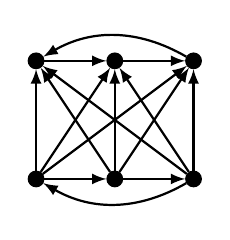
\begin{tikzpicture}
    \node[draw, circle, fill=black, inner sep=2pt] at (-1, 0.75) (a) {};
    \node[draw, circle, fill=black, inner sep=2pt] at (0, 0.75) (b) {};
    \node[draw, circle, fill=black, inner sep=2pt] at (1, 0.75) (c) {};
    \node[draw, circle, fill=black, inner sep=2pt] at (-1, -0.75) (d) {};
    \node[draw, circle, fill=black, inner sep=2pt] at (0, -0.75) (e) {};
    \node[draw, circle, fill=black, inner sep=2pt] at (1, -0.75) (f) {};
    \draw[-latex,thick] (d) -- (e);
    \draw[-latex,thick] (e) -- (f);
    \draw[-latex,thick] (f) to[bend left] (d);
    \draw[-latex,thick] (a) -- (b);
    \draw[-latex,thick] (b) -- (c);
    \draw[-latex,thick] (c) to[bend right] (a);
    \foreach \x in {a,b,c} {
      \foreach \y in {d,e,f} {
        \draw[-latex,thick] (\y) -- (\x);
      }
    }
  \end{tikzpicture}
\end{center}
\begin{proposition}
  $\varphi(K_n) = 3$ for all even $n\geq 6$.
\end{proposition}
\begin{proof}
  The base case $n=6$ is proven above.
  Let $n\geq 6$ and suppose this is true for $n$.
  \begin{center}
    \begin{tikzpicture}
      \node[draw, circle, fill=black, inner sep=2pt] at (1, 1) (x) {};
      \node[draw, circle, fill=black, inner sep=2pt] at (-1, 1) (y) {};
      \node[ellipse, draw, minimum height=1cm, minimum width=4cm, fill=red!10, label=right:$K_n$] at (0, 0) {};
      \node[draw, circle, fill=black, inner sep=2pt] at (-1.5, 0) (a) {};
      \node[draw, circle, fill=black, inner sep=2pt] at (-0.5, 0) (b) {};
      \node[draw, circle, fill=black, inner sep=2pt] at (0.5, 0) (c) {};
      \node[draw, circle, fill=black, inner sep=2pt] at (1.5, 0) (d) {};
      \draw[thick] (x) -- (y);
      \foreach \x in {x,y} {
        \foreach \y in {a,b,c,d} {
          \draw[thick] (\x) -- (\y);
        }
      }
    \end{tikzpicture}
  \end{center}
  To show that $\varphi(K_{n+2}) = 3$, it suffices by induction to show that
  $K_{2,n}^+$ has a nowhere-zero $\bZ_3$ flow, where $K_{2,n}^+$ is
  \begin{center}
    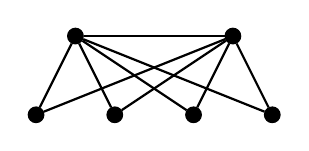
\begin{tikzpicture}
      \node[draw, circle, fill=black, inner sep=2pt] at (1, 1) (x) {};
      \node[draw, circle, fill=black, inner sep=2pt] at (-1, 1) (y) {};
      \node[draw, circle, fill=black, inner sep=2pt] at (-1.5, 0) (a) {};
      \node[draw, circle, fill=black, inner sep=2pt] at (-0.5, 0) (b) {};
      \node[draw, circle, fill=black, inner sep=2pt] at (0.5, 0) (c) {};
      \node[draw, circle, fill=black, inner sep=2pt] at (1.5, 0) (d) {};
      \draw[thick] (x) -- (y);
      \foreach \x in {x,y} {
        \foreach \y in {a,b,c,d} {
          \draw[thick] (\x) -- (\y);
        }
      }
    \end{tikzpicture}
  \end{center}
  that is, a $K_{2,n}$ with an edge added between the vertices in the size-2 part.

  Let $x,y$ be the vertices in all the triangles of $K_{2,n}^+$
  (i.e. the size-2 part).
  Let $z$ be a common neighbour of $x,y$.
  This gives the following diagram.
  \begin{center}
    \begin{tikzpicture}
      \node[draw, circle, fill=black, inner sep=2pt, label=left:$x$] at (-1, 1) (x) {};
      \node[draw, circle, fill=black, inner sep=2pt, label=right:$y$] at (1, 1) (y) {};
      \node[draw, circle, fill=black, inner sep=2pt, label=above:$z$] at (0, 1.5) (z) {};
      \node[ellipse, draw, minimum height=1cm, minimum width=4cm, fill=red!10, label=right:$K_{n-1}$] at (0, 0) {};
      \node[draw, circle, fill=black, inner sep=2pt] at (-1.5, 0) (a) {};
      \node[draw, circle, fill=black, inner sep=2pt] at (-0.5, 0) (b) {};
      \node[draw, circle, fill=black, inner sep=2pt] at (0.5, 0) (c) {};
      \node[draw, circle, fill=black, inner sep=2pt] at (1.5, 0) (d) {};
      \draw[thick] (x) -- (y) -- (z) -- (x);
      \foreach \x in {x,y} {
        \foreach \y in {a,b,c,d} {
          \draw[thick] (\x) -- (\y);
        }
      }
    \end{tikzpicture}
  \end{center}
  Define a flow $\varphi$ of $K_{2,n}^+$ by orienting $x\to w$ and $w\to y$ for
  all $w\notin\{x,y,z\}$ and then orienting $xy,xz,yz$ accordingly.
  \begin{center}
    \begin{tikzpicture}
      \node[draw,circle,fill=black,inner sep=2pt,label=left:$x$] at (-1, 1) (x) {};
      \node[draw,circle,fill=black,inner sep=2pt,label=right:$y$] at (1, 1) (y) {};
      \node[draw,circle,fill=black,inner sep=2pt,label=above:$z$] at (0, 1.5) (z) {};
      \node[ellipse,draw,minimum height=1cm,minimum width=4cm,fill=red!10,label=right:$K_{n-1}$] at (0, 0) {};
      \node[draw,circle,fill=black,inner sep=2pt] at (-1.5, 0) (a) {};
      \node[draw,circle,fill=black,inner sep=2pt] at (-0.5, 0) (b) {};
      \node[draw,circle,fill=black,inner sep=2pt] at (0.5, 0) (c) {};
      \node[draw,circle,fill=black,inner sep=2pt] at (1.5, 0) (d) {};
      \draw[thick] (x) -- (z) -- (y) -- (x);
      \foreach \y in {a,b,c,d} {
        \draw[-latex, thick] (x) -- (\y);
        \draw[-latex, thick] (\y) -- (y);
      }
    \end{tikzpicture}
  \end{center}
  The orientation depends on the value of $n\bmod 3$; the cases are
  $x\gets y\gets z\gets x$, $x\to y\gets z\gets x$, and $x\gets y\to z\to x$.
\end{proof}
\begin{question*}
  Is $\varphi(G)\geq 4$ for some bridgeless $G\neq K_4$?
\end{question*}
We can look at 3-regular graphs.
\begin{proposition}
  If $G$ is 3-regular, then $\varphi(G) = 4$ iff $G$ is 3-edge-colourable.
\end{proposition}
\begin{proof}
  Note that $G$ has a nowhere-zero $\bZ_4$-flow iff $G$ has a nowhere-zero
  $\bZ_2\times\bZ_2$ flow.
  \begin{proposition}
    \mnote{The $\Gamma_1\times\Gamma_2$-flow is the \textit{product} of the
    $\Gamma_1$-flow with the $\Gamma_2$-flow.}%
    $G$ has a nowhere-zero $\Gamma_1\times\Gamma_2$-flow iff $G$ has a
    $\Gamma_1$-flow $\varphi_1$ and a $\Gamma_2$-flow $\varphi_2$ such that
    no edge satisfies $\varphi_1(e) = \varphi_2(e) = 0$.
  \end{proposition}
  If $\varphi$ is a nowhere-zero $\bZ_2\times\bZ_2$-flow in a cubic (i.e. 3-regular)
  graph $G$, then for each vertex $v$, the edges at $v$ must all be assigned
  different flow values by $\varphi$ (otherwise there exist $e_1,e_2$ at $v$
  with $\varphi(e_1) = \varphi(e_2)$ so
  $\varphi(e_3) = -\varphi(e_1) - \varphi(e_2) = 0$ for the third edge $e_3$).
  Now $\varphi$ is a 3-edge-colouring (your colours are the non-zero elements
  of $\bZ_2\times\bZ_2$).
\end{proof}
Because the above is an iff, we want a cubic graph that is not 3-edge-colourable.
Consider the Peterson graph:
\begin{center}
  \begin{tikzpicture}
    \foreach \x in {1,2} {
      \foreach \t/\y in {0/a,1/b,2/c,3/d,4/e} {
        \node[draw,circle,fill=black,inner sep=2pt] at
          ($({0.75*\x*sin(360*\t/5)},{0.75*\x*cos(360*\t/5)})$) (\y\x) {};
      }
    }
    \foreach \y in {a,b,c,d,e} {
      \draw[thick] (\y1) -- (\y2);
    }
    \draw[thick] (a1) -- (c1) -- (e1) -- (b1) -- (d1) -- (a1);
    \draw[thick] (a2) -- (b2) -- (c2) -- (d2) -- (e2) -- (a2);
  \end{tikzpicture}
\end{center}

Note that it has girth 5, so if it were 3-edge-colourable, it would have to be
the union of 3 matchings.
Then consider the union of two colour classes: this is a 2-regular graph and so
must be either a cycle or the union of cycles.
Because the girth is 5, if it is the union of cycles, it must be the union of
two 5-cycles, but 5-cycles are not 2-edge-colourable.
Finally, it can be shown that the graph is not Hamiltonian and so it is not
3-edge-colourable.
\begin{exercise*}
  Show the Peterson graph has a nowhere-zero $\bZ_5$-flow.
\end{exercise*}
Recall there is an 8-flow theorem from matroid theory.
There is a stronger result by Seymour.
\begin{theorem}[Seymour '81]
  Every bridgeless graph has a nowhere-zero 6-flow.
\end{theorem}
We need the following propositions.
\begin{proposition}
  If $G$ is bridgeless, then so is $G/C$ for each $C\subseteq E(G)$.
\end{proposition}
\begin{proof}
  Proof omitted (simple proof by matroid theory: take the dual; now deleting
  edges cannot produce loops).
\end{proof}\begin{proposition}
  Let $S\subseteq E(G)$.
  \begin{enumerate}[label=(\arabic*)]
    \item Every flow on $G/S$ extends to a flow on $G$.

    \item If $S$ induces a connected subgraph of $G$, and $u$ is the
      corresponding contracted vertex of $G/S$, and $\varphi'$ is a flow on
      $G/S$ with $\varphi'(e) = 0$ for all $e\in\delta(u)$, and $\varphi_S$ is a
      flow on $G[S]$, then $\varphi'\cup\varphi_S$ is a flow on $G$.
      % There was a diagram here but I got rid of it since I don't think it's useful.

    \item If $\Gamma$ is a group with $|\Gamma|\geq 3$ and $S$ is a set of
      at least 2 parallel edges, then every $\Gamma$-flow $\varphi'$ on $G/S$
      extends to a $\Gamma$-flow $\varphi$ on $G$ such that $\varphi(e)\neq 0$
      for all $e\in S$.
  \end{enumerate}
\end{proposition}
\begin{proof}
  On assignment.
\end{proof}
The 6-flow theorem follows from the following claim.
\begin{claim}
  For every bridgeless oriented graph $G$ and every vertex $u\in V(G)$,
  there is a nowhere-zero $(\bZ_2\times\bZ_3)$-flow $\varphi_2\times\varphi_3$
  such that $\varphi_2(e) = 0$ for all $e\in\delta(u)$.
\end{claim}
\begin{proof} \lecture{Thu Nov 23}%
  Induct on $|V(G)|$.
  Let $u\in V(G)$.
  If $|V(G)| = 1$, the graph is just loops (which cancel themselves).
  \begin{itemize}
    \item \textbf{Case 0:} $u$ has only loops.

      Induct on $G - u$.

    \item \textbf{Case 1:} $G - u$ has a bridge $e$.

      \begin{center}
        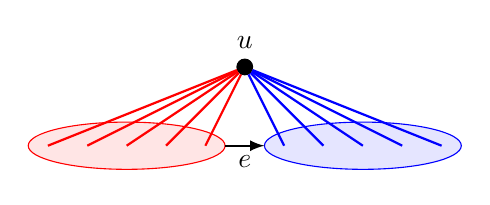
\begin{tikzpicture}
          \node[draw,circle,fill=black,inner sep=2pt, label=above:$u$] (u) at (0, 0) {};
          \draw[red,fill=red!10] (-1.5, -1) circle(1.25cm and 0.3cm);
          \draw[blue,fill=blue!10] (1.5, -1) circle(1.25cm and 0.3cm);
          \draw[thick,-latex] (-0.25, -1) -- node[below]{$e$} (0.25, -1);
          \foreach \x in {0.5, 1, ..., 2.5} {
            \draw[red, thick] (u) -- (-\x, -1);
            \draw[blue, thick] (u) -- (\x, -1);
          }
        \end{tikzpicture}
      \end{center}
      Let $E_1\cup E_2\cup\{e\}$ be an associated partition of $E(G)$.
      For each $i$, let $G_i = G/E_i$ with contracted vertex $u$.

      {\hspace*{\fill}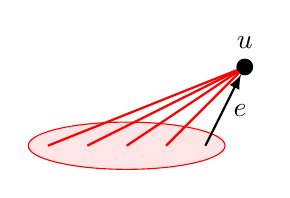
\begin{tikzpicture}
        \node[draw,circle,fill=black,inner sep=2pt, label=above:$u$] (u) at (0, 0) {};
        \draw[red,fill=red!10] (-1.5, -1) circle(1.25cm and 0.3cm);
        \foreach \x in {1, 1.5, ..., 2.5} {
          \draw[red, thick] (u) -- (-\x, -1);
        }
        \draw[thick, -latex] (-0.5, -1) -- node[right]{$e$} (u);
      \end{tikzpicture}\hspace*{\fill}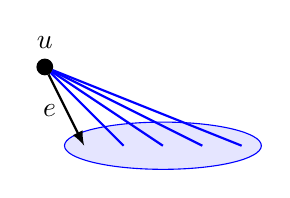
\begin{tikzpicture}
        \node[draw,circle,fill=black,inner sep=2pt, label=above:$u$] (u) at (0, 0) {};
        \draw[blue,fill=blue!10] (1.5, -1) circle(1.25cm and 0.3cm);
        \foreach \x in {1, 1.5, ..., 2.5} {
          \draw[blue, thick] (u) -- (\x, -1);
        }
        \draw[thick, -latex] (u) -- node[left]{$e$} (0.5, -1);
      \end{tikzpicture}\hspace*{\fill}}

      In particular, note that the $G_i$ must be of the above form because $G$
      is bridgeless, so $e$ cannot be a bridge in $G$ and thus $u$ must be
      incident to both $E_i$.

      Inductively, each $G_i$ has a nowhere-zero $\bZ_2\times\bZ_3$-flow
      $\varphi^i = \varphi^i_2\times\varphi^i_3$ such that
      $\varphi_2^i|_{\delta_{G_i}(u)}\equiv 0$.
      Note that $\varphi^i(e)\in\{(0,1),(0,2)\}$ for each $i$.
      By possibly replacing $\varphi^i$ with $-\varphi^i$, we may assume that
      $\varphi^1(e) = \varphi^2(e)$.
      So $\varphi = \varphi^1\cup\varphi^2$ is a function with domain $E(G)$.

      This is clearly a nowhere-zero pre-flow.
      For each $x\neq u$, if $x\in V(G_i)$ then
      $\Delta_\varphi(x) = \Delta_{\varphi^i}(x) = 0$.
      Since $\varphi$ is a pre-flow, $\sum_{x\in V(G)}\Delta_\varphi(x) = 0$,
      thus it follows that $\Delta_{\varphi}(u) = 0$.
      Thus $\varphi$ is a flow on $G$ and
      $\varphi|_{\delta(u)}\equiv 0$ by construction.

    \item \textbf{Case 2:} $G - u$ is bridgeless.

      Since $G$ is bridgeless, there are distinct edges $e_1 = ux_1, e_2 = ux_2$
      (possibly with $x_1 = x_2$) at $G$ such that $x_1,x_2$ are in the same
      component of $G - u$ (take a cycle through $u$).

      Let $H$ be a connected even subgraph of $G - u$ containing $x_1$ and $x_2$
      (e.g. the union of two edge-disjoint $x_1x_2$-paths in $G - u$.
      Let $S$ be the set of edges from $u$ to $V(H)$.

      Let $G' = G/E(H)$ with contracted vertex $x$.
      Let $G'' = G'/S$ with contracted vertex $u$.
      Inductively, $G''$ has a nowhere-zero $\bZ_2\times\bZ_3$-flow
      $\varphi_2''\times\varphi_3''$ such that
      $\varphi_2''|_{\delta_{G''}(u)}\equiv 0$.

      Let $\varphi_2^S$ be the flow on $G'[S]$ that is identically zero.
      By (2), since $\varphi_2''|_{\delta(u)}\equiv 0$, the function
      $\varphi_2' = \varphi_2''\cup\varphi_2^S$ is a $\bZ_2$-flow on $G'$.

      By (3), since $|S|\geq 2$, and $|\bZ_3|\geq 3$, there is an extension
      of $\varphi_3''$ to a $\bZ_3$-flow $\varphi_3'$ on $G'$ such that
      $\varphi_3'(e)\neq 0$ for all $e\in S$.

      Now let $\varphi_2^H$ be the $\bZ_2$-flow on $H$ that is everywhere 1.
      This is a flow because every vertex has even degree in $H$.
      Since $\varphi_2'|_{\delta(x)}\equiv 0$, by (2), the function
      $\varphi_2'\cup\varphi_2^H$ is a $\bZ_2$-flow on $G$.

      By (1), there is an extension $\varphi_3$ of $\varphi_3'$ to a
      $\bZ_3$-flow on $G$.
      Now $\varphi_2$ is nonzero on $E(H)$, $\varphi_3$ is nonzero on $S$,
      and $\varphi_2\times\varphi_3$ is equal to $\varphi_2''\times\varphi_3''$
      on $E(G) - (E(H)\cup S)$, so is nonzero.
      It follows that $\varphi_2\times\varphi_3$ is a nowhere-zero
      $(\bZ_2\times\bZ_3)$-flow.

      Finally, by construction, $\varphi_2|_{\delta(u)}\equiv 0$
      (consider edges in $S$ and edges outside $S$ separately). \qedhere
  \end{itemize}
\end{proof}
This doesn't extend easily to the 5-flow conjecture,
because all known proofs of the 6-flow theorem use $\bZ_6\cong\bZ_2\times\bZ_3$
but $\bZ_5$ admits no such decomposition.
\begin{conjecture}
  Every bridgeless graph has a nowhere-zero 5-flow.
\end{conjecture}
\subsection{Flows and Planarity}
\begin{theorem}
  \th\label{thm:planar-dual-flow-color}
  If $G$ and $H$ are dual planar embeddings then $\varphi(G) = \chi(H)$.
\end{theorem}
We need the following definition.
\begin{definition*}[Arc, arc function]
  An \vocab{arc} of an undirected (multi)graph $G$ is an ordered triple
  $(e;x,y)$ such that $x,y$ are the ends of $e$.
  Each non-loop edge gives two arcs.
  Let $A(G)$ be the set of arcs of $G$.
  An \vocab{arc function} of $G$ is a function $\varphi:A\to\Gamma$,
  where $\Gamma$ is abelian, such that $\varphi(e;x,y) = -\varphi(e;y,x)$ for all
  arcs $(e;x,y)$.
  Given a set $X$ of arcs, write $\varphi(X)$ for $\sum_{a\in X}\varphi(a)$.
\end{definition*}
This is equivalent to the definition of arc given in the textbook.
\begin{exercise*}
  A loopless graph $G$ has a nowhere-zero $\Gamma$-flow iff $G$ has a
  nowhere-zero arc function $\varphi$ such that
  $\sum_{e\in\delta(x_0)}\varphi(e;x_0,y) = 0$ for all $x_0\in V$.
\end{exercise*}
With the above exercise we can now prove \th\ref{thm:planar-dual-flow-color}.
\begin{proof}[Proof of \th\ref{thm:planar-dual-flow-color}]
  We may assume that $G$ and $H$ are 2-connected, so faces of $G$ correspond
  to vertices of $H$ and vice-versa.
  Let $\Gamma$ be an abelian group.
  If $G$ has a nowhere-zero $\Gamma$-flow, let $\psi$ be the associated arc
  function.
  Define an arc function $\pi$ on $E(H)$ as shown:
  \begin{center}
    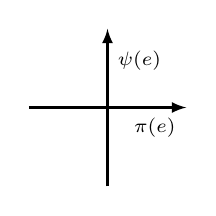
\begin{tikzpicture}
      \draw[-latex,thick](-1,0) -- (1,0) node[pos=0.8,anchor=north]{\scriptsize$\pi(e)$};
      \draw[-latex,thick](0,-1) -- (0,1) node[pos=0.8,anchor=west]{\scriptsize$\psi(e)$};
    \end{tikzpicture}
  \end{center}
  Then the fact that $\psi$ came from a flow implies that $\pi(C) = 0$ for
  every directed facial cycle of $H$.
  Thus the fact that $\psi$ came from a flow implies that $\psi(\delta^+(v)) = 0$
  so $\pi(C) = 0$.

  Then by induction, $\pi(C) = 0$ for every directed cycle of $H$.
  This implies that for every pair of $vw$-walks $P_1,P_2$ in $H$,
  one has $\pi(P_1) = \pi(P_2)$.
  If we fix $v_0\in V(H)$ and define $c:V(H)\to\Gamma$ by
  $c(x) = \pi(\text{some $v_0x$-walk})$ then $c$ is a $\Gamma$-colouring of $H$.
  This means $\chi(H)\leq\varphi(G)$.

  Conversely, given a proper colouring $c$ of $H$,
  define an arc function $\phi$ of $G$ as follows:
  \begin{center}
    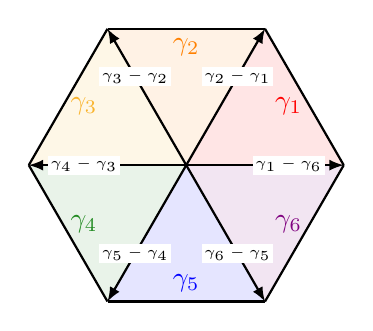
\begin{tikzpicture}
      \foreach \x/\y in {0/red,1/orange,2/Dandelion,3/ForestGreen,4/blue,5/violet}{
        \fill[\y!10]({2*cos(60*\x)},{2*sin(60*\x)})--({2*cos(60*(\x+1))},{2*sin(60*(\x+1))})--(0,0);
        \draw[thick] ({2*cos(60*\x)},{2*sin(60*\x)})--({2*cos(60*(\x+1))},{2*sin(60*(\x+1))});
      }
      \foreach \x/\y in {1/2,2/3,3/4,4/5,5/6,6/1}{
        \draw[-latex, thick] (0,0)--({2*cos(60*\x)},{2*sin(60*\x)}) node[pos=0.65,fill=white,inner sep=1pt]{\tiny$\gamma_\y-\gamma_\x$};
      }
      \foreach \x/\y in {1/red,2/orange,3/Dandelion,4/ForestGreen,5/blue,6/violet}{
        \node[\y] at ({1.5*cos(60*\x-30)},{1.5*sin(60*\x-30)}) {$\gamma_{\x}$};
      }
    \end{tikzpicture}
  \end{center}
  Note that this is a flow, because summing the outgoing edges gives 0.
  As $c$ is a proper colouring, no two adjacent vertices of $H$ have the same
  colour, and so $\phi$ is a nowhere-zero $\chi(H)$-flow.
\end{proof}
\begin{remark*}
  This gives a correspondence between 4-colourings in the primal graph
  and 3-edge-colourings in the dual.
\end{remark*}

\end{document}

